\documentclass[11pt]{article}
\usepackage[utf8]{inputenc}
\usepackage[T1]{fontenc}
\usepackage[francais]{babel}
\usepackage[top=2.5cm, bottom=2.5cm, left=2.5cm, right=2.5cm]{geometry}
\usepackage{hyperref}   % Sommaire PDF
\usepackage{graphicx}   % Insertion d'images
\usepackage{multirow}   % Fusion de cellules de tableaux
\usepackage{float}      % Placement des figures
\usepackage{xcolor}     % Couleurs
\usepackage{eurosym}    % Symbole €

% En-tête, pied-de-page
\usepackage{fancyhdr}
\pagestyle{fancy}
\renewcommand{\headrulewidth}{0pt}
\lhead{}
\chead{}
\rhead{}
\lfoot{}
\cfoot{\thepage}
\rfoot{}

\begin{document}
    \title{Droit}
    \author{Christine MAKSSOUD}
    \date{}

% Page de garde + page blanche
\maketitle
\setcounter{page}{0} \thispagestyle{empty} % Ne pas numéroter la page de garde + pas d'en-tête/pied-de-page
\newpage
\setcounter{page}{2} % Commencer la numérotation à 2

\newpage
~\\
\renewcommand{\contentsname}{Sommaire}
\tableofcontents

% Début du document
\newpage
\part{Les fonctions de droit et la règle de droit}
	Le droit est fonction de régulation sociale. Il organise la société au nom de certaines valeurs. Il est aussi connaissance et objet d'étude. Sa fonction symbolique est aussi reconnue.
	
	\section{La notion de droit}
		\subsection{Définition}
			Le droit est l'ensemble des règles qui régissent la vie des hommes en société. Un non-respect entraine des sanctions. Omniprésent dans la vie des individus, il permet l'organisation de la vie sociale.
			
		\subsection{Légitimité}
			Seules les règles créées par une autorité légitime sont des règles de droit. Le droit a une légitimité :
				\begin{itemize}
					\item juridique : la règle de droit est instituée par une autorité investie du pouvoir de la créer (parlement, gouvernement, maires,...). Elle peut être le fruit d'une concertation entre l'autorité publique et les groupes de pression, ou de la négociation entre partenaires sociaux;
					\item sociale : la règle de droit organise la société et les rapports des hommes entre eux.
				\end{itemize}
				
		\subsection{Diversité}
			Les juristes distinguent le droit objectif, qui est l'ensemble des règles applicables dans un état. Le droit objectif détermine l'ensemble des droits subjectifs. Il s'agit de déterminer la part de liberté et de contraintes de chacun. Il faut définir ce qui est permis ou pas pour que la vie sociale soit possible. Lorsqu'on étudie la règle de droit objectif, cela signifie qu'on prend en considération la règle de droit en elle-même et pour elle-même, abstraction faite de son contenu. On envisage ce qui est commun à toutes les règles juridiques, ses caractères, ses classifications, ses sources, son domaine d'applicaton,...
			
			Les droits subjectifs sont des prérogatives dont une personne peut se prévaloir sur un bien ou sur une autre personne. Ces prérogatives sont assorties d'obligation attribuées à une personne par le droit objectif. Avec les droits subjectifs, on peut faire ou exiger quelque chose.
			
	\section{Les fonctions de droit}
		\subsection{Organiser la vie}
			Le droit organise la vie en société au nom de certaines valeurs : la recherche de la justice, de la sécurité et de la légalité.
			
		\subsection{Réguler la vie en société}
			Le droit a pour objectif de civiliser les relations sociales. Il remplace les rapports de force par des rapports de droit. Le droit assure à tous les hommes un statut de sujet de droit libres et égaux.
			
		\subsection{Traduire des valeurs collectives}
			Le Droit est la traduction de valeurs collectives, c'est à dire d'idéaux que les membres d'une société partagent et qu'ils entendent promouvoir. Par exemple, liberté, égalité, affirmé par la constitution, « tous les hommes naissent libres et égaux en droits ». La solidarité, être jeune et moins jeune, est prévue par la sécurité sociale. La laïcité est affirmée par l'article L141-5 du Code de l'Éducation.
			
			L'évolution du système de valeurs entraine une modification de la règle de droit. La règle de droit peut aussi contribuer à faire évoluer les modes de pensée et d'action. Par exemple, la loi Évin du 10/01/1991 visant à lutter contre le tabagisme et l'alcoolémie.
			
	\section{Les caractères de la règle de droit}
		\subsection{Le caractère général et abstrait}
			La règle de droit est générale. Elle s'applique sans distinction à tous les citoyens et à certaines catégories de citoyens, mais pas à une personne en particulier. La généralité de la règle est une garantie contre toute discrimination personnelle. Par exemple, les principes d'égalité des citoyens devant la loi, les emplois publics, et les charges publiques (préambule de la constitution de 1958, déclaration universelle des droits de l'Hommet et du Citoyen de 1789).
			
			La règle de droit est abstraite. Elle ne vise aucune personne déterminée, mais cela ne s'applique qu'à ceux appartenant à la catégorie ou à la situation visée. C'est pourquoi sa formulation est impersonnelle. Par exemple, l'article 488 du Code Civil affirme « la majorité est fixée à 18 ans accomplis. On est capable de tous les actes de la vie civile. » Cette règle ne vise personne en particulier, mais elle est destinée à tous ceux qui ont atteint l'âge de 18 ans. À ce titre, les mots quiconque, chacun, le fait de, sont souvent employées.
			
		\subsection{Le caractère obligatoire}
			La règle de droit est obligatoire. Nul ne peut déroger à la loi, dès lors qu'il entre dans son champ d'application. Parce qu'il est sensé la connaître, le citoyen ne peut justifier faire entorse à la loi par sa méconnaissance de la règle. « Nul n'est censé ignorer la loi ». La règle de droit est assortie de sanctions, de peines diverses, qui dépendent de la nature de la règle de droit. Par exemple, au pénal, il peut s'agir d'une amende ou d'une peine de prison. Au civil, ce peut être le paiement de dommages et intérêts à la victime, destinés à réparer le préjudice accusé, annulation d'un contrat, exécution forcée,...
			
			On dit que la règle de droit à un caractère coercitif, c'est à dire que les pouvoirs publics peuvent utiliser la force publique pour faire respecter une règle de droit et peuvent condamner un manquement à l'obligation de la respecter.

\newpage
\part{Les droits fondamentaux}
	\section{Les principes et les droits fondamentaux}
		La France est une démocratie. L'autorité vient du peuple. Les principes démocratiques sont énoncés par la constitution de 1958 et contenus dans la devise « Liberté, égalité, fraternité ». La citoyenneté liée à la démocratie recouvre les droits civiles et politiques, et les devoirs incombant aux citoyens. Les droits fondamentaux et les garanties des citoyens sont définies dans les lois, notamment pour les libertés individuelles, et leurs applications contemporaines.
		
	\section{Les droits et les devoirs des citoyens}
		Les droits de l'Homme se sont enrichis avec la création récemment de droits à l'environnement.
		\begin{itemize}
			\item Première génération : droits naturels reconnus à tout être humain, droits fondamentaux et libertés individuelles (droit à la vie, dignité, sûreté, propriété,...);
			\item Deuxième génération : garanties matérielles (droit économiques, sociaux et culturels);
			\item Troisième génération : nouvelle catégories de droits constitutionnels, droits à un environnement propre et sain
		\end{itemize}
		
		Les droits s'accompagnent de devoirs et d'obligations accomplies par les citoyens pour le bien de la nation et définis dans les lois.
		
		
	\section{La protection des libertés et les restrictions}
		L'état doit assurer les garanties des libertés dans le respect de la démocratie. Les lois doivent s'adapter (mondialisation des échanges de données, nouvelles technologies d'identification,...). En cas d'atteinte à leurs libertés, les citoyens peuvent saisir selon les cas les tribunaux chargés de l'application de la loi ou la CNIL\footnote{Commission Nationale Informatique et Liberté : protège la vie privée et les libertés individuelles et publiques. Elle contrôle les nouvelles technologies, joue un rôle d'alerte et donne des conseils aux citoyens pour exercer leurs droits ou porter plainte. La CNIL peut prononcer des sanctions pour non-respect de la loi.}. Des organisations humanitaires ou publiques veillent au respect des droits de l'Homme au niveau international. Des restrictions des libertés individuelles sont parfois prises par les pouvoirs publics pour des raisons d'intérêt général ou d'ordre public et la recherche d'une sécurité collective grandissante et plus efficace.

\newpage
\part{Les sources du droit}
	Les droits ont été établis par des autorités diverses, et des habitudes qui sont établies. Certaines règles sont internationales dû à l'adhésion de la France à des traités ou conventions internationaux, d'autres communautaires (UE). Les sources du droit sont diverses, hiérarchisées et complémentaires.

	\section{Les sources écrites du droit}
		\subsection{Les sources nationales}
			\subsubsection{La constitution}
				C'est un ensemble de textes (Déclaration des Droits de l'Homme et du Citoyen) de 1789, préambule de 1946 et consolidation du 14/08/1958. Ces textes organisent le partitionnement des institutions et la répartition qui affirme les grandes libertés et les grands principes qui fondent notre système juridique. La constitution du 4/10/58 est le texte fondateur de la 5\up{ème} République. La constitution peut être modifiée par voie de référendum ou par le parlement. Le Conseil Constitutionnel peut être saisi par les députés ou les sénateurs pour étudier des lois en discussion et vérifier leur conformité par rapport à la constitution, qui est le texte de référence. C'est la source la plus importante en droit interne.
	
			\subsubsection{Les lois}
				Une loi est une règle juridique écrite, votée par le parlement (Assemblée Nationale et Sénat) qui détient le pouvoir législatif. La loi s'applique après promulgation du Président de la République et parution au Journal Officiel.
				
				La liste des matières qui relèvent du domaine de la loi est définie par l'article 34 de la constitution, elles sont totalement régies par la loi : droit civique, libertés publiques, définition des crimes, délits et peines. Dans d'autres matières, elle ne détermine que les principes fondamentaux, les règles d'application étant fixées par décret. La loi est obligatoire est permanente.

				\begin{figure}[h!]
					\begin{center}
						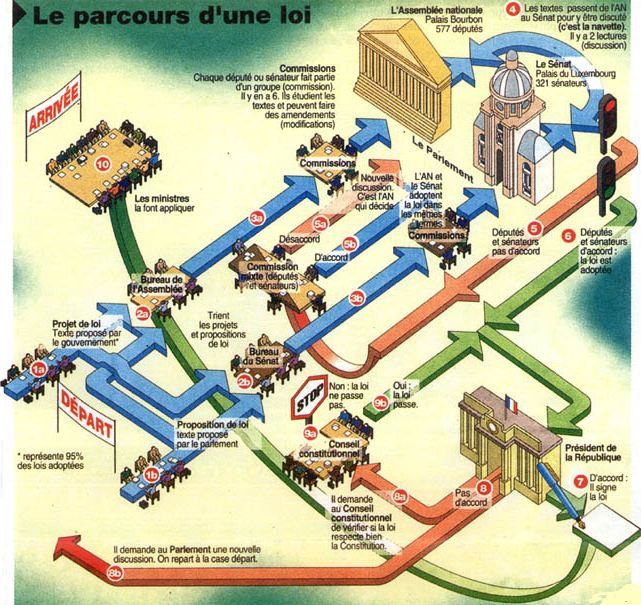
\includegraphics[scale=0.7]{images/ParcoursLoi.png}
						\caption{Parcours d'une loi}
					\end{center}
				\end{figure}
				
			\subsubsection{Les règlements}
				Les règlements sont des textes élaborés par les pouvoirs exécutifs. Certains règlements sont établis pour préciser les conditions de mise en œuvre d'une loi. Ce sont des décrets d'application. On parle d'arrêté quand ces règlements sont élaborés par un ministre, préfet ou maire.
				
			\subsubsection{Les ordonnances}
				Le gouvernement peut demander au parlement l'autorisation de prendre des mesures juridiques qui relèvent normalement du domaine législatif. C'est un texte élaboré par le pouvoir exécutif mais entrant dans le domaine de la loi. Les ordonnances sont décidées en conseil des ministres, et une fois ratifiées par le parlement ont valeur de loi.
				
		\subsection{Les sources internationales}
			\subsubsection{Les traités}
				Les traités sont des accords conclus entre la France et divers pays étrangers sur des domaines très variés (commerce, industrie, ...). Ils peuvent prendre différentes formes : bilatéraux (entre deux pays), conventions douanières, traité d'organisation de la vie économique,... Les traités ratifiés ont une autorité supérieure à celle des lois et ils jouent un rôle croissant parmi les sources du droit.
				
			\subsubsection{Le droit européen}
				On distingue le droit européen primaire, qui correspond aux différents traités à l'origine de l'Union Européenne, et le droit européen dérivé, élaboré par les instances européennes. Il y a deux normes : le règlement et la directive.
				
				Le règlement est la loi européenne par excellence. Elle a force obligatoire dans chaque état membre. Un état ne peut se soustraire à son exécution. Il est d'application immédiate. 	La directive lie tout état membre quand à son résultat à atteindre, elle laisse aux instances nationales la compétence quant à la forme et au moyen. Elle indique le délai dont disposent les états membres pour prendre les mesures internes nécessaires. Les règlements et directives sont élaborés par la commission européenne à Bruxelles et adoptés par le conseil des ministres en co-décision avec le parlement européen à Strasbourg. Le droit communautaire l'emporte toujours sur le droit français.
				
	\section{Les sources non-écrites de droit}
		\subsection{La jurisprudence}
			La jurisprudence est l'œuvre de l'autorité judiciaire. C'est l'ensemble des décisions rendues par les tribunaux sur un point de droit litigieux. Deux conditions : la répétition et la hiérarchie. Il arrive qu'une seule décision fasse jurisprudence lorsqu'elle émane d'une juridiction d'un très haut niveau dans la hiérarchie judiciaire (cours de cassation,...).
			
			La jurisprudence est du droit dans le sens où elle interprète les lois, elle comble les lacunes de la loi et fait évoluer les droits. Les jurisprudences ne sont pas définitives car les juges peuvent toujours changer d'avis en raison de l'évolution des pratiques des citoyens.
			
		\subsection{Les coutumes et les usages}
			La coutume est une règle de droit née d'une pratique habituelle et prolongée considérée par certains comme obligatoire, à condition de ne pas aller à l'encontre de la loi. Les usages sont des règles professionnelles et locales qui s'imposent par le caractère répété et la croyance en leur caractère obligatoire.
			
			Les coutumes et les usages ne sont pas des règles écrites, elles peuvent disparaître.
			
		\subsection{La doctrine}
			C'est l'ensemble des travaux des auteurs qui expriment leur conception théorique et commentent les lois. La doctrine ne s'impose jamais aux juges mais peut les influencer.
			
	\section{La hiérarchie des sources de droit}
		\begin{figure}[h!]
			\begin{center}
				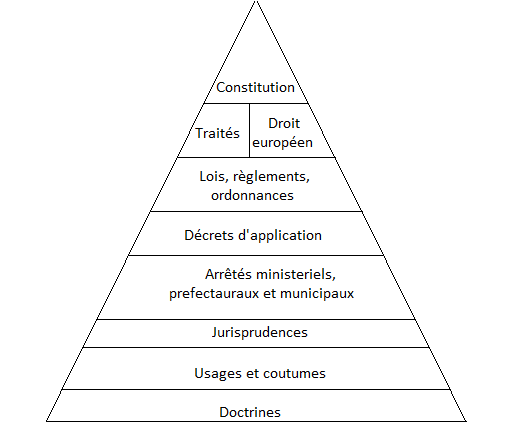
\includegraphics{images/HierarchieSourcesDroit.png}
				\caption{Hiérarchie des sources de droit}
			\end{center}
		\end{figure}
		
		Chaque texte de niveau inférieur doit être compatible avec ceux qui lui sont supérieurs dans la hiérarchie.
		
	\section{Les titulaires des droits subjectifs}
		\subsection{La notion de personnalité juridique}
			La loi définit la personnalité juridique comme étant l'aptitude à être titulaire de droits et d'obligations. On distingue les personnes physiques des personnes morales.
			
		\subsection{Les personnes physiques}
			\subsubsection{Les personnes physiques}
				On appelle personne physique tout individu auquel la loi donne des droits et des obligations. Elle est reconnue de la naissance à la morte de tout être humain.
				
				Ces droits sont inséparables de la personne et ne peuvent pas être vendus sans aucune valeur pécuniaire. Les atteintes au droit de la personnalité peuvent faire l'objet de poursuites pénales et donner lieu à réparation des préjudices subis.
				
			\subsubsection{L'identification des personnes physiques}
				\paragraph{Le nom de famille} Depuis la loi du 1\up{er} janvier 2005, tout enfant pourra recevoir soit le nom de sa mère, soit celui de son père, ou des deux dans l'ordre choisi.
				
				\paragraph{Le domicile} Le lieu du principal établissement de la personne.
				
				\paragraph{La nationalité} La liaison juridique de rattachement d'un individu à un état. En France, la nationalité peut être obtenue grâce au :
					\begin{itemize}
						\item Droit du sol (naissances en France
						\item Mariage (depuis le 24/07/2006, un étranger uni à un citoyen français depuis 4 ans obtient la nationalité française
						\item Naturalisation : un étranger peut demander la nationalité française
						\item Droit du sang : naissance de parents français
					\end{itemize}
					
				\paragraph{Le patrimoine} L'ensemble des obligations du contribuable en argent (droits pécuniaires et dettes).
			
			\subsubsection{La capacité des personnes physiques}
				\paragraph{La capacité juridique} Les individus sont considérés comme ayant une aptitude générale à participer à la vie juridique.
					\subparagraph{La capacité de jouissance} L'aptitude à être titulaire de droits et débiteur d'obligations. On est titulaire de droits dès la naissance.
					
					\subparagraph{La capacité d'exercice} L'aptitude à exercer les droits dont on est titulaire, acquise à la majorité. Les sujets sont dits capables.
					
				\paragraph{L'incapacité juridique}
					\subparagraph{L'incapacité de jouissance} Elle prive la personne incapable de certains droits. Il s'agit de condamner la personne qui a eu un comportement susceptible de porter atteinte à l'ordre public.
					
					\subparagraph{L'incapacité d'exercice} Une personne titulaire de droits mais ne pouvant les exercer seules pour des raisons liées à l'âge, à l'altération des facultés physiques ou mentales de cette personne est dite incapable d'exercice. Le but est de protéger le patrimoine de la personne incapable qui doit être assistée par un représentant légal.
				
				\paragraph{La protection des personnes physiques}
					\subparagraph{Sauvegarde de justice} Mesure de protection temporaire destinée à protéger une personne majeure, tout ou partie de son patrimoine, si elle n'a plus la capacité de le faire seule. Elle conserve sa capacité et l'exercice de ses droits.
					
					\subparagraph{La curatelle} Le patrimoine du majeur est confié à un curateur désigné par le juge des tutelles quand il a besoin d'être assisté au contrôle de ses biens de manière continue.
					
					\subparagraph{La tutelle} Mesure juridique destinée à protéger une personne majeure et tout ou partie de son patrimoine si elle n'est plus en état de veiller sur ses propres intérêts. Le tuteur peut la représenter dans les actes de la vie sociale.
					
					\subparagraph{Mandat de protection future} L'objectif est de protéger les personnes vulnérables. C'est un contrat qui permet à une personne d'organiser à l'avance sa protection ou celle de son enfant handicapé en choisissant celui ou celle qui sera chargé de s'occuper de ses affaires le jour où elle ne pourra plus le faire en raison de son âge ou de son état de santé.
					
		\subsection{Les personnes morales}
			\subsubsection{Les personnes morales}
				C'est un groupement de personnes auquel est attribué la personnalité juridique afin de leur permettre de mettre en commun leurs moyens au service d'une activité professionnelle ou pour représenter et défendre leurs intérêts collectifs. Leurs droits sont exercés par des personnes physiques qui les représentent.
				
				\paragraph{Naissance de la personne morale} Immatriculation au registre du commerce, préfecture, mairie. Elle peut avoir un objet lucratif ou non lucratif. La personnalité juridique des personnes morales prend fin à sa dissolution.
				
				\paragraph{Personne morale de droit privé} société, association, syndicat, fondations et groupements d'intérêts économiques.
				
				\paragraph{Personne morale de droit public} État, collectivités, établissements publics
				
			\subsubsection{Identification}
				\begin{itemize}
					\item dénomination sociale (société), titre (association)
					\item siège social
					\item nationalité
					\item capital
				\end{itemize}
				
			\subsubsection{La capacité des personnes morales}
				Elle est limitée à l'objet décidé par les personnes physiques qui ont rédigé les statuts. Les personnes morales n'ont pas le droit de vote. La capacité d'exercice ne peut se réaliser que par l'intermédiaire d'une personne physique qui passera des contrats ou signera au nom de la personne morale.
\end{document}
